\section{StatsBombR - Descrizione pratica}
        Nella sezione corrente, verranno descritti tre esempi pratici, di difficoltà e interesse crescente. L'obiettivo è quello di utilizzare, per quanto possibile, le conoscenze apprese durante il corso. Per rendere intuitiva e precisa la presentazione, si è scelto di descrivere gli esempi mescolando una parte di spiegazione e una parte di codice R, senza scendere troppo nei dettagli tecnici. Nella presentazione, laddove il codice risultasse ripetitivo, o privo di rilevante significato, lo si ometterà. Ad ogni modo, in fondo al documento, si possono trovare i codici degli esempi proposti, in blocco. Per ogni applicazione, alla fine, si effettueranno alcuni ragionamenti critici sui risultati e sui grafici ottenuti.
        
        \subsection{Esempio 1}
            Il primo esempio che si vuole proporre ha principalmente lo scopo di familiarizzare con le funzioni messe a disposizione dalla libreria StatsBombR, quindi non ha una particolare valenza strategica dal punto di vista delle football analytics. Si vuole mostrare, mediante uno scatterplot, la relazione tra la media stagionale d'impiego del noto calciatore Lionel Messi (nato nel 1987), espressa dal minutaggio e le competizioni a cui egli ha partecipato (principalmente compionati, tornei e coppe), nel corso della sua carriera. Le competizioni saranno per la maggior parte campionati, quindi coinvolgeranno annate calcistiche. Si anticipa che lo script astrae dai club per i quali il giocatore in questione ha militato nell'arco della sua carriera, com'è giusto che sia.   

            Come prima cosa, si esegue il pull delle competizioni di qualsiasi annata e zona geografica. Successivamente, si salvano, in una lista di data-frame \texttt{SplitSeasons}, tutte le gare relative a ogni competizione.

            \vspace{5pt}
            
            \begin{lstlisting}[numbers=None]
    library(ggplot2)
    library(StatsBombR)
    
    
    Comp <- FreeCompetitions()
    
    Matches <- FreeMatches(Comp) %>%
      group_by(season.season_id)
      
    SplitSeasons <- group_split(Matches)
            \end{lstlisting}

            In seguito, per ogni competizione, si estraggono tutti i minuti giocati da Messi (id giocatore 5503) e gli eventi legati alle partite di quella particolare competizione. Un evento è un'azione che ha senso essere registrata nell'arco di una partita, come per esempio un tiro, un passaggio, un goal. Una cosa importante da ricordare è che se si prova a richiamare la funzione della libreria per l'estrazione degli eventi \texttt{StatsBombFreeEvents()}, produce un errore, simile a quello riportato in figura \ref{fig:StatsBombFreeevents}. La soluzione è sostituire tale funzione con la funzione \texttt{free\_allevents()}. Maggiori dettagli si possono trovare qui \cite{StatsBombFreeEventsError}, in una issue aperta a tale proposito nella repository GitHub.

            \begin{figure}[h]
                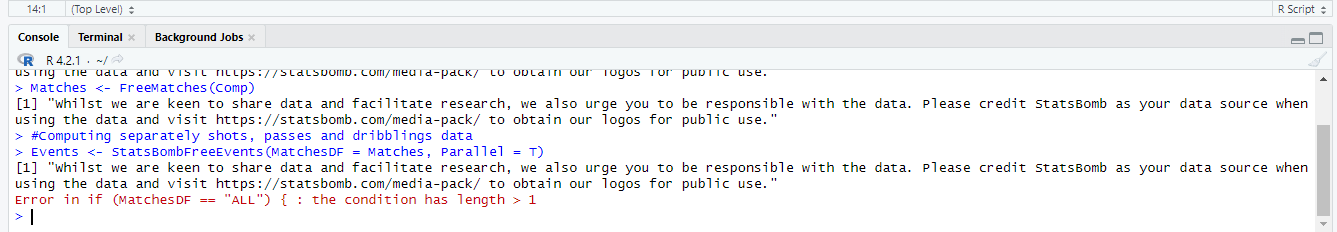
\includegraphics[scale=0.3]{StatsBombFreeEventsError.png}
                \centering
                \caption{Errore nella funzione StatsBombFreeEvents()}
                \label{fig:StatsBombFreeevents}
            \end{figure}
            
            Per ogni competizione, si calcolano i minuti totali giocati e il numero di partite. In seguito viene calcolata anche la media del minutaggio riferita a ogni competizione e, si riversano i dati raccolti in coda al dataframe \texttt{MessiMinutesSeason}, inizialmente vuoto. Infine si ordina per anno relativo a ciascuna competizione, in senso crescente, il dataframe. Si ricorda che se si prova a eseguire il codice seguente, richiede qualche minuto per essere portato a termine. Dopo il codice, per avere un'idea, si riporta in figura \ref{fig:MessiMinutesSeason} il dataframe \texttt{MessiMinutesSeason}.

            \vspace{5pt}

            \begin{lstlisting}[numbers=None]
    #Pulling down Lionel Messi minutes in all seasons, then we sort the dataframe with ascendant order, based on season
    MessiMinutesSeason <- data.frame()
    
    for (i in (1:length(SplitSeasons))) {
      Events <- free_allevents(MatchesDF = SplitSeasons[[i]], Parallel = T)
      Events <- formatelapsedtime(Events)
      MessiMinutesPlayed <- get.minutesplayed(Events) %>%
        filter(player.id == 5503) %>%
        summarise(player.id = 5503,
                  season = unique(SplitSeasons[[i]]$season.season_name),
                  tot.minutes = sum(MinutesPlayed),
                  matches = n(),
                  avg.minutes = tot.minutes / matches)
      if (MessiMinutesPlayed$matches > 0) {
        MessiMinutesSeason <- rbind(MessiMinutesSeason, MessiMinutesPlayed)
      }
    }
    
    MessiMinutesSeason <- MessiMinutesSeason %>%
      arrange(season)
    
    view(MessiMinutesSeason)
            \end{lstlisting}

            \begin{figure}[h]
                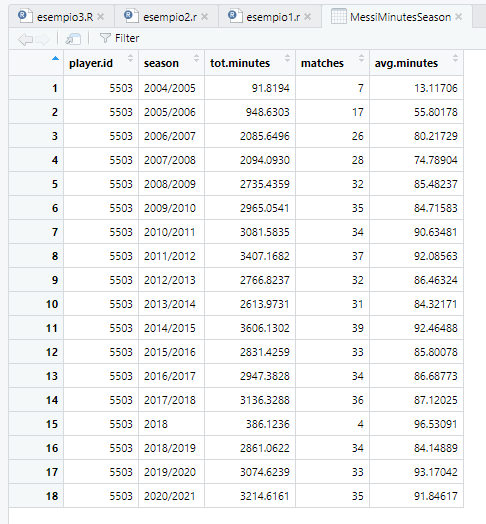
\includegraphics[height=4cm, width=5cm]{immagini/MessiMinutesSeason.png}
                \centering
                \caption{Dataframe MessiMinutesSeason}
                \label{fig:MessiMinutesSeason}
            \end{figure}

            Infine, si procede a plottare i risultati, richiamando la funzione \texttt{ggplot()} del pacchetto ggplot2, specificando i parametri grafici riportati.

            \begin{lstlisting}[numbers=None]
    #Now we can finally plot results
    ggplot(MessiMinutesSeason, mapping=aes(x=season, y=avg.minutes, group=1)) +
      geom_line(color="blue") +
      geom_point() +
      geom_text(aes(x=season, y=avg.minutes, label=matches),size = 2.5, nudge_y = 2, nudge_x = -0.05) +
      ylab('Media minuti per partita') + 
      xlab('Annata competizione calcistica')
            \end{lstlisting}

            In figura \ref{fig:plot1} vi è il grafico risultante e, anche se può sembrare contro-intuitivo, si è deciso di aggiungere un'etichetta ai punti del grafico, con il fine di aumentarne l'espressività. Ciascuna etichetta indica il numero di partite giocate da Messi in una determinata competizione, quindi, a titolo d'esempio, nel corso campionato  2017/2018, egli ha partecipato a 36 gare, con una media di 87.12 minuti a partita. 
            
            Analizzando la curva mostrata, si può notare che è abbastanza simile a quella attesa, dal momento che nel 2003/2004 il giocatore aveva appena 16 anni e, per quanto fosse un top-player già all'epoca, è naturale pensare che il suo impiego non sia stato alto. D'altronde, quale allenatore farebbe pesante affidamento su un giocatore giovane e inesperto? Proseguendo l'analisi, si può notare che da un certo punto in poi, invece, l'impiego, oltre ad essere cresciuto, si è più o meno stabilizzato, raggiungendo un picco di massimo ai mondiali in Russia nel 2018 (96 minuti a partita). Tale picco non è particolarmente significativo, dal momento che riflette abbastanza chiaramente i difetti che ha la media, in quanto, per definizione, a un mondiale vi sono molte meno partite (dati) disputabili rispetto a un campionato. In particolare Messi ha disputato 4 partite, praticamente per intero (una partita dura 90 minuti più recupero), con la conseguente media d'impiego alta. Si è preferito lasciare le competizioni separate per chiarezza, in quanto vi sarebbe l'incertezza nell'addensare le partite dei mondiali al campionato 2017/2018 o al campionato 2018/2019. Si noti infine che il calciatore è stato molto fortunato nel corso della sua carriera, dal momento che sembra aver subito pochissimi infortuni, dal momento che ha disputato molte partite.

            \begin{figure}[h]
                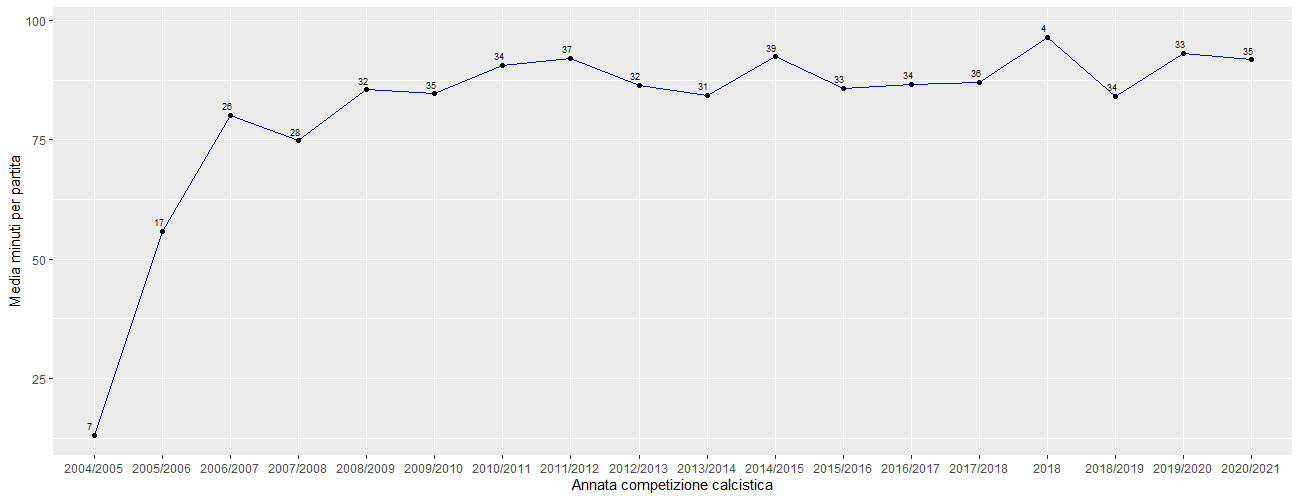
\includegraphics[height=5cm,width=\textwidth]{Rplot01.png}
                \centering
                \caption{Scatterplot annata competizione calcistica vs. media minutaggio}
                \label{fig:plot1}
            \end{figure}

        \newpage

        \subsection{Esempio 2}
            L'esempio che si propone ora è certamente più interessante rispetto al precedente, dal punto di vista dell'analisi dei dati. L'idea è di proporre un grafico che tenga conto dei passaggi, dei tiri e dei dribbling (un dribbling è un'azione che si ritiene tale quando si supera un avversario senza perdere il possesso della palla). Ciò che si vuole evidenziare, in verità, è qualcosa di più espressivo: si vuole mostrare qual è la propensione di un giocatore a tirare, passare la palla a un compagno o a dribblare. In altri termini, quali sono le scelte che egli opera quando è in possesso di palla. 
            
            Per fare ciò, si rappresentano le tre dimensioni (nel caso in esame valori percentuali) tramite un ternary plot, ovvero sia un grafico a forma di triangolo equilatero che consente di esprimere, lungo ciascun lato (asse) del triangolo, le tre variabili che sommano tutte a un valore costante, tipicamente 1 o, come nella situazione corrente, 100. 
            
            Si propongono diverse applicazioni di tale grafico, la cui funzione è contenuta e richiamabile dal pacchetto ggtern e, prima di cominciare a descrivere l'esempio, si vuole dare un'idea di lettura del grafico. Esistono tre modi equivalenti di trovare i valori di un punto nel grafico, descritti tutti in \cite{TernaryPlot}. 
            
            Il modo più semplice è probabilmente quello relativo alle linee parallele ai lati del triangolo, di cui un esempio si può trovare in figura \ref{fig:lettura}. Nella prima figura, è presente la scala percentuale di limo via via crescente verso l'alto e che taglia "a fette" il grafico orizzontalmente. Nella seconda figura, si può notare la scala percentuale di argilla via via crescente verso il basso e che taglia "a fette" il grafico in senso obliquo verso destra. Infine nella terza figura, si può notare la scala percentuale di sabbia via via crescente verso destra e che taglia "a fette" il grafico in senso obliquo verso destra. Chiaramente, l'intersezione dei tre segmenti determina i valori (coordinate) percentuali di un punto.

            \begin{figure}[h]
                \makebox[\textwidth][c]{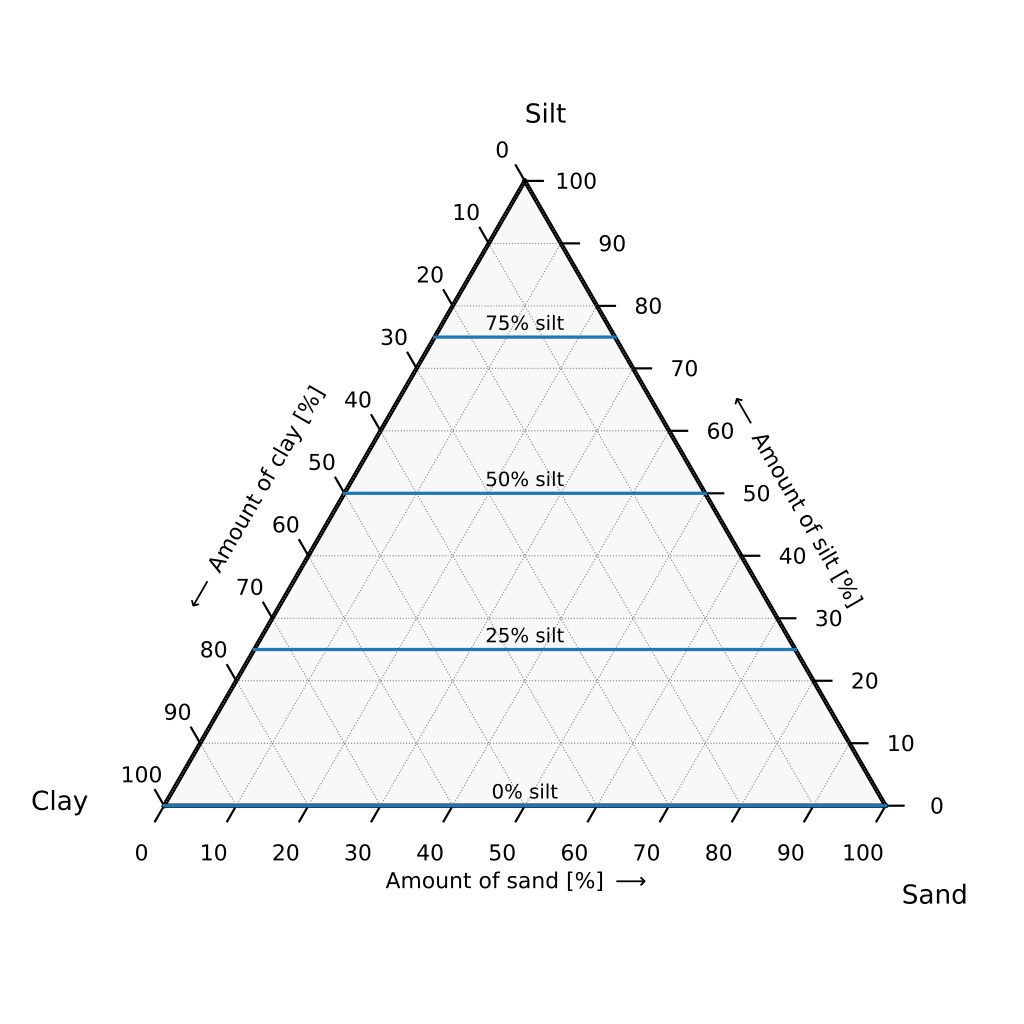
\includegraphics[width=0.425\textwidth]{t1.png}
                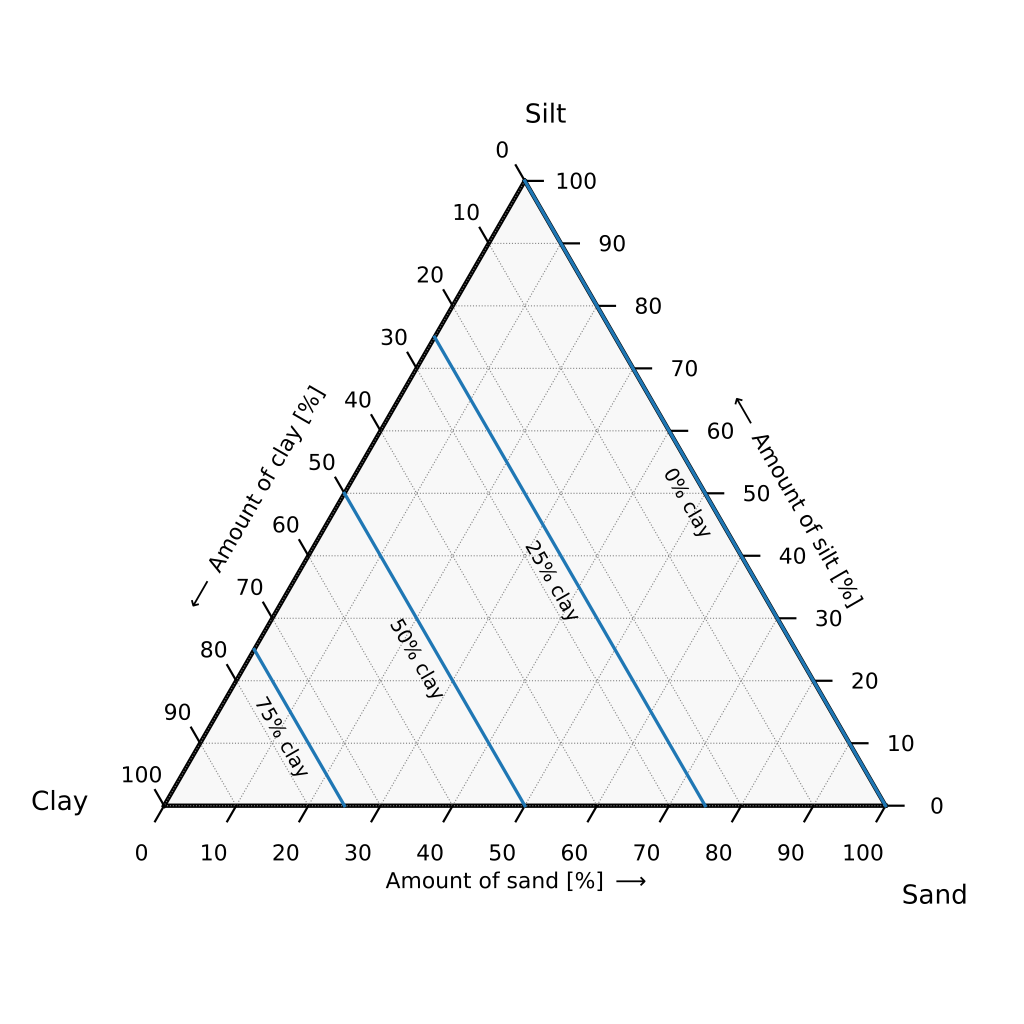
\includegraphics[width=0.425\textwidth]{t2.png}
                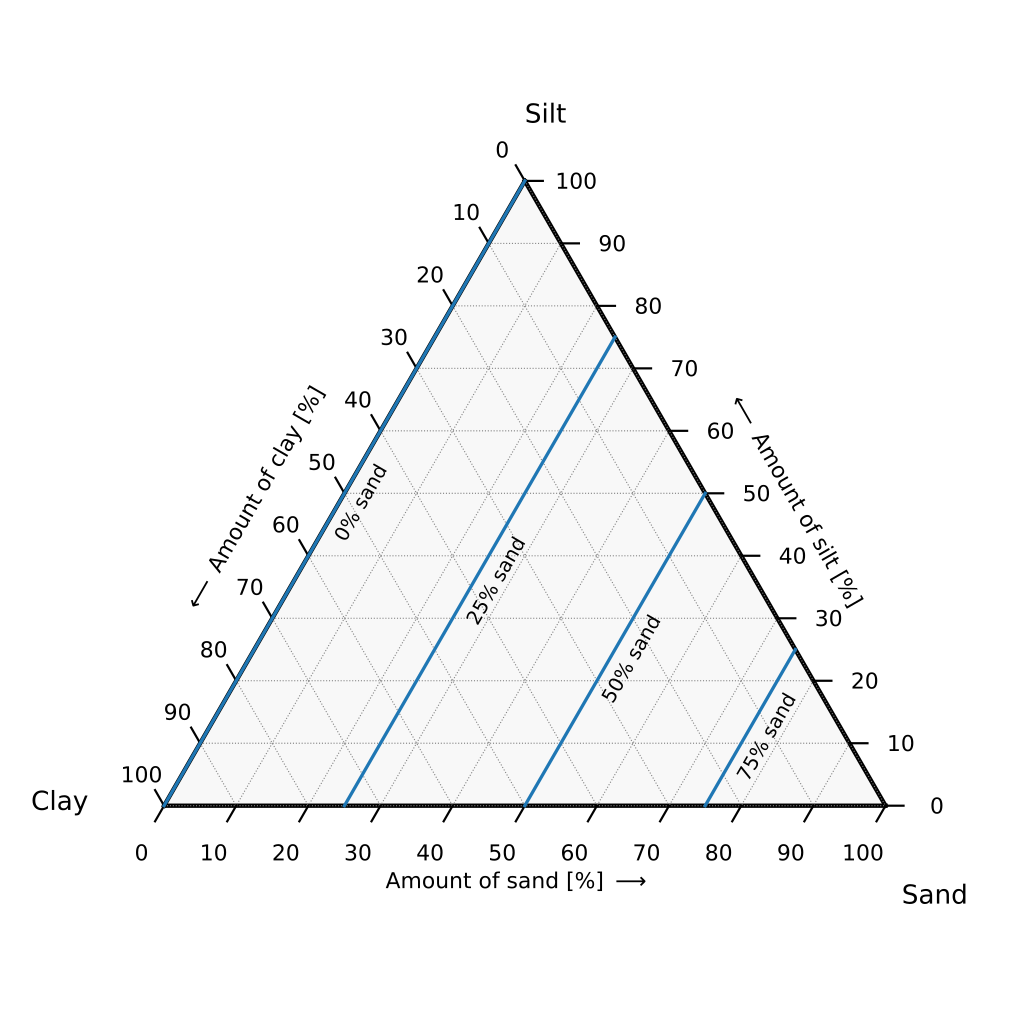
\includegraphics[width=0.425\textwidth]{t3.png}}
                \caption{Lettura del ternary plot}\label{fig:lettura}
            \end{figure}

            A questo punto, una volta introdotto il ternary plot, si può cominciare presentando l'esempio. Inizialmente si estrae l'annata calcistica "2020/2021" del campionato spagnolo "La Liga" e tutte le partite relative a tale stagione.

            \vspace{5pt}

            \begin{lstlisting}[numbers=None]
    library(ggtern)
    library(StatsBombR)
    
    
    #Filtering season by competition (Spain - La Liga) and season_id (2020/21)
    Comp <- FreeCompetitions() %>%
      filter(competition_id == 11 & season_id == 90)
    
    Matches <- FreeMatches(Comp)
            \end{lstlisting}
            
            \vspace{5pt}

            In seguito, si scaricano gli eventi legati alle partite della stagione sopra menzionata (escludendo gli eventi non associati ad alcun giocatore) e si calcolano i tiri, i passaggi e i dribbling che hanno un relativo id.
            
            \vspace{5pt}
            
            \begin{lstlisting}[numbers=None]
    #Computing separately shots, passes and dribblings data
    Events <- free_allevents(MatchesDF = Matches, Parallel = T) %>%
      allclean() %>%
      filter(player.name != "NA") %>%
      group_by(player.name, team.name)
    
    Shots <- Events %>%
      filter(shot.type.id != "NA") %>%
      count(player.name)
    colnames(Shots)[3] = "n.shots"
    
    Passes <- Events %>%
      filter(pass.type.id != "NA") %>%
      count(player.name)
    colnames(Passes)[3] = "n.passes"
    
    Dribblings <- Events %>%
      filter(dribble.outcome.id != "NA") %>%
      count(player.name)
    colnames(Dribblings)[3] = "n.dribblings"
    
    Results <- data.frame(unique(Events$player.name))
    colnames(Results)[1] = "player.name"
            \end{lstlisting}

            \vspace{5pt}

            Non rimane che calcolare le percentuali relative alle tre dimensioni che vogliamo rappresentare nel grafico e unire i due dataframe \texttt{Results} e \texttt{Percent}. Per avere un'idea, in figura \ref{fig:Results}, si mostra una parte del dataframe \texttt{Results} dopo l'unione. Si noti che tutte le percentuali sommano a 100.

            \vspace{5pt}

            \begin{lstlisting}[numbers=None]
    #Merging Shots, Dribblings and Passes in Results, keeping players who played in the same team the whole year
    Results <- Results %>%
      left_join(Shots, by = "player.name") %>%
      left_join(Passes, by = "player.name") %>%
      left_join(Dribblings, by = "player.name") %>%
      na.omit() %>%
      filter(team.name.x == team.name.y & team.name.y == team.name & team.name == team.name.x) %>%
      select(-team.name.y, -team.name)
    
    #Computing percentages of shots, dribblings and passes and then we merge them again in Results 
    Percent <- data.frame()
    for (i in 1:nrow(Results)) {
      Tmp <- Results[i, 3] + Results[i, 4] + Results[i, 5]
      PercS <- (Results[i, 3] / Tmp) * 100
      PercP <- (Results[i, 4] / Tmp) * 100
      PercD <- (Results[i, 5] / Tmp) * 100
      SumPerc <- PercS + PercP + PercD
      Values <- c(Tmp, PercS, PercP, PercD, SumPerc)
      Percent <- rbind(Percent, Values)
    }
    
    Results <- cbind(Results, Percent)

    colnames(Results) <- c("player.name", "team.name", "n.shots", "n.passes", "n.dribblings", 
                      "tot.sum", "p.shots", "p.passes", "p.dribblings", "tot.p.sum")

    head(Results)
            \end{lstlisting}
            
            \begin{figure}[h]
                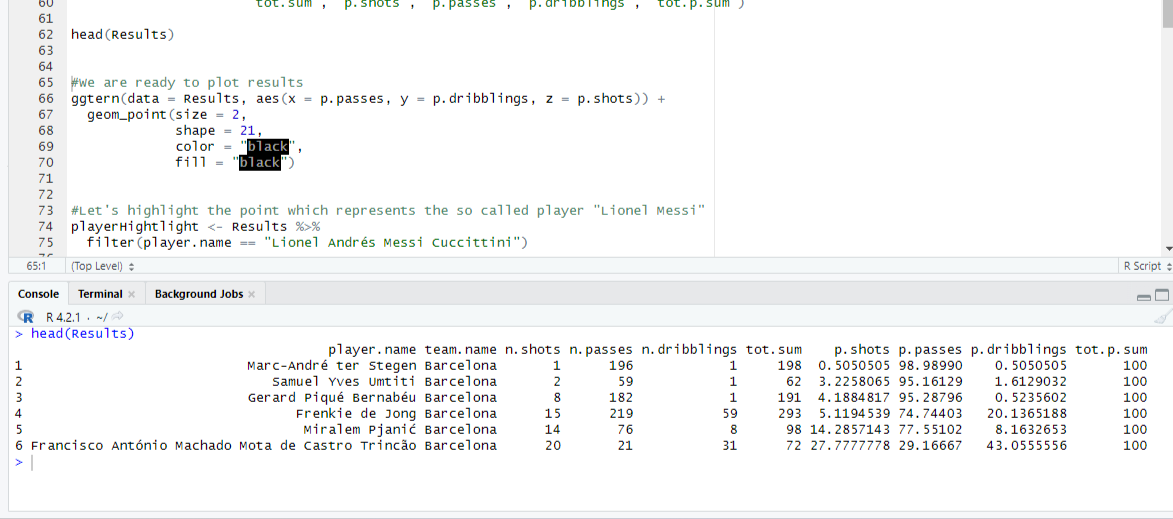
\includegraphics[height=4cm,width=\textwidth]{Results.png}
                \centering
                \caption{Dataframe Results}
                \label{fig:Results}
            \end{figure}

            A questo punto, si è pronti a mostrare qualche grafico. Per evitare di tediare il lettore, si è scelto di non presentare alcun codice qui, in quanto abbastanza ripetitivo e ricco di funzioni in cui vengono specificati principalmente i parametri grafici. In figura \ref{fig:ternary} sono presenti 4 versioni del ternary plot: 
            
            Nella prima in alto a sinistra, sono rappresentati tutti i calciatori del campionato spagnolo (2020/2021). Si può subito notare che i punti rappresentati tendono ad addensarsi nella parte in basso a sinistra del grafico, indice del fatto che tanti giocatori effettuano molti passaggi, pochi dribbling e pochissimi tiri. Questo fatto non è da considerarsi anomalo, in quanto il passaggio della palla a un compagno è sicuramente un gesto tecnico più semplice e frequente rispetto a un tiro o a un dribbling. Per convicersi, è sufficiente pensare che il passaggio può essere effettuato in ogni zona del campo, mentre un dribbling o un tiro, solitamente, hanno senso se effettuati dalla metà campo avversaria in poi. Appurato ciò, non sono da escludersi situazioni anomale in cui, per esempio, i dati disponibili riguardano principalmente giocatori che tirano o dribblano poco, oppure i dati registrati tengono conto principalmente dei passaggi, quindi si hanno poche informazioni sui tiri o sui dribbling. 
            
            Nella seconda figura in alto a destra, sono stati selezionati i giocatori "Lionel Messi" (attaccante) e "Marc-André ter Stegen" (portiere). Per quanto riguarda Messi, il punto si trova leggermente spostato in basso a sinistra, rispetto al centro del grafico, segno del fatto che il giocatore ha complessivamente, un ottimo equilibrio tra le tre dimensioni considerate, con una leggere prevalenza dei passaggi rispetto alle altre due variabili. Tipicamente per un giocatore che ha un ruolo come il suo, ovvero di attaccante, ci si aspetta che il punto sia spostato verso la dimensioni tiro e/o dribbling. In questo caso, la quasi centralità, può voler dire che il giocatore sia molto coinvolto dalla squadra nella manovra dell'azione e magari che la sua posizione sia spesso lontana dalla porta avversaria. Per quanto riguarda invece il portiere ter Stegen, egli rispecchia un comportamento normale, in quanto il punto si trova praticamente sul vertice basso a sinistra, indice del fatto che effettua quasi solo passaggi.
            
            Nella figura in basso a sinistra, sono stati evidenziati tutti i calciatori della squadra "Barcelona", anch'essi confermano la tendenza al passaggio, come tutti gli altri calciatori del campionato spagnolo della figura in alto a sinistra e pertanto valgono all'incirca le stesse considerazioni fatte. Ci si aspetta quindi che i calciatori più vicini al vertice basso sinistro abbiano i ruoli di portiere e difensore, mentre più ci si allontana, più avranno i ruoli di centrocampista e attaccante, anche se questa ipotesi non è sempre vera, come nel caso di Messi.
            
            \begin{figure}[h]
                \makebox[\textwidth][c]{\includegraphics[width=0.425\textwidth]{RPlot02.png}
                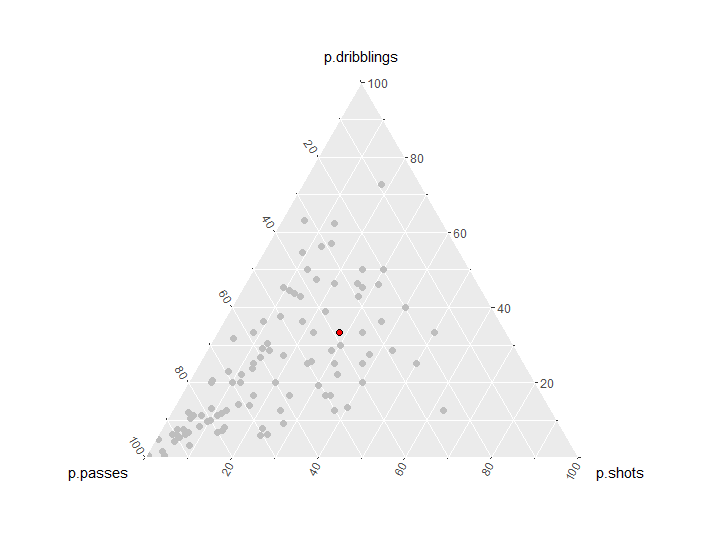
\includegraphics[width=0.425\textwidth]{Rplot03.png}}
                \makebox[\textwidth][c]{\includegraphics[width=0.425\textwidth]{RPlot04.png}
                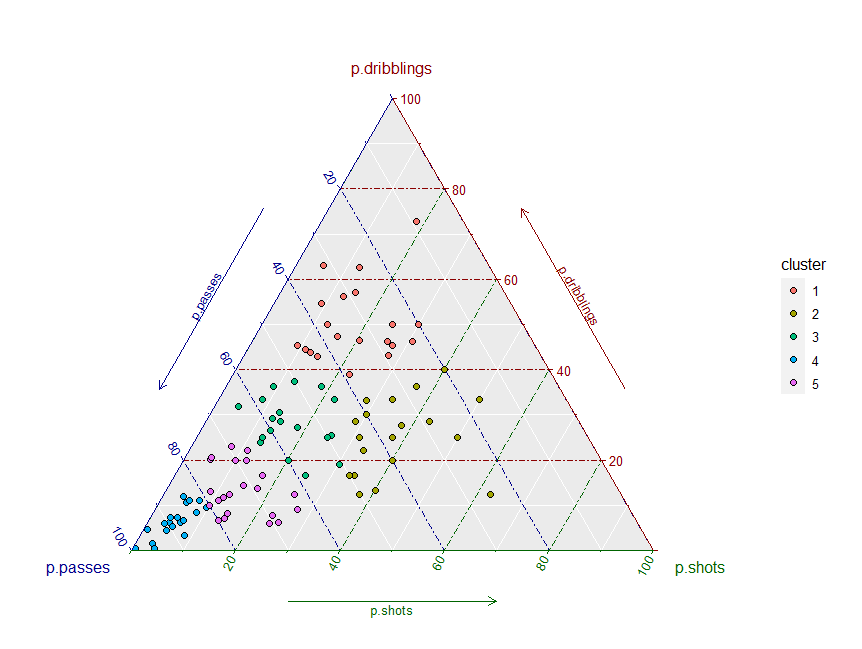
\includegraphics[width=0.425\textwidth]{Rplot05.png}}
                \caption{Applicazioni del ternary plot}\label{fig:ternary}
            \end{figure}

            Infine, l'ultima figura in basso a destra merita un focus particolare. Ciò che si vuole proporre è un partizionamento in 5 gruppi (il numero dei gruppi è arbitrario) dei calciatori del campionato spagnolo (2020/2021), sfruttando la procedura di partizionamento in clusters k-means, di cui si possono avere maggiori dettagli qui \cite{K-means}. Come mostrato in maniera più chiara in figura \ref{fig:Clustering}, i giocatori appartenenti al gruppo 4 hanno una tendenza a passare la palla maggiore all'80\%. Questi raggruppamenti, in uno scenario ipotetico, potrebbero risultare molto utili in ottica di calciomercato, dal momento che una squadra potrebbe trovarsi a dover vendere un giocatore appartenente a tale gruppo e per l'amministrazione, non sarebbe difficile trovare un sostituto senza rompere gli equilibri della squadra, dal momento che sarebbe sufficiente comprarne un altro che appartenga anch'esso al gruppo 4.

            \begin{figure}[h]
                \includegraphics[scale=0.5]{RPlot05.png}
                \centering
                \caption{Clustering tramite k-means}
                \label{fig:Clustering}
            \end{figure}

            Ad esempio, se la squadra Barcelona dovesse trovarsi costretta a vendere il giocatore "Sergio Busquets i Burgos", posizionato al quarto posto come tendenza a passare la palla del cluster 4 (figura \ref{fig:ReplacePlayer}), potrebbe facilmente rimpiazzarlo con "Carlos Henrique Casimiro" (Real Madrid) o con "Martín Zubimendi Ibáñez" (Real Sociedad), rispettivamente all'ottavo e nono posto del medesimo cluster. 
            
            Volendo spingersi oltre con l'analisi, magari considerando variabili aggiuntive, come per esempio l'età del giocatore, la percentuale di riuscita dei passaggi o altro ancora, dal momento che al giorno d'oggi le squadre di calcio professionistiche sono considerate delle vere e proprie aziende, potrebbe essere altrettanto utile per il Barcelona vendere "Sergio Busquets i Burgos" e rimpiazzarlo con un giocatore appartenente al gruppo 5 (tendenza al passaggio tra circa il 60\% e l'80\%), con l'obiettivo di migliorare le sue qualità, per esempio. Probabilmente un giocatore di tale gruppo costerebbe meno rispetto a uno del gruppo 4 perchè, come detto sopra, basterebbe acquistare un giocatore più giovane e quindi più inesperto, permettendo al Barcelona di realizzare un profitto dalla vendita. Chiaramente, tali ragionamenti sono in questo contesto, fini a se stessi, avendo a disposizione una mole di dati molto bassa, sebbene siano tutti dati reali. Tuttavia, sono ragionamenti molto interessanti che vale la pena fare.
            
            \vspace{10pt}
            
            \begin{figure}[h]
                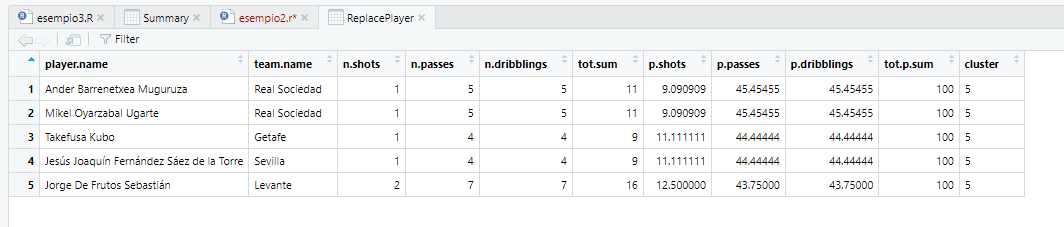
\includegraphics[scale=0.6]{ReplacePlayer.png}
                \centering
                \caption{Dataframe ReplacePlayer}
                \label{fig:ReplacePlayer}
            \end{figure}
            
        
        \subsection{Esempio 3}
            Per il terzo e ultimo esempio, si propone inizialmente la rappresentazione tramite scatterplot della media tiri e goal segnati per partita dei calciatori del campionato inglese, relativo alla stagione 2003/2004. Si porrà l'attenzione su una regione dello scatterplot, con l'obiettivo di rappresentare in un ulteriore grafico i tiri e i goal effettuati dai calciatori, rappresentati da punti colorati diversamente, presenti nella medesima zona dello scatterplot, evidenziando anche alcune metriche utilizzate al giorno d'oggi nelle football analytics.

            Al solito, si estrae la competizione di interesse, ovvero il campionato inglese (Premier League), la cui unica season disponibile è quella legata all'annata 2003/2004, le relative partite e gli eventi legati ad ogni partita.

            \vspace{10pt}

            \begin{lstlisting}[numbers=None]
    library(ggrepel)
    library(ggplot2)
    library(ggsoccer)
    library(StatsBombR)
    
    
    #Considering all the seasons available in the English championship (Premier League)
    Comp <- FreeCompetitions() %>%
      filter(competition_id == 2)
    
    Matches <- FreeMatches(Comp)
    
    Events <- free_allevents(MatchesDF = Matches, Parallel = T) %>% 
      allclean()
            \end{lstlisting}

            \vspace{10pt}
            
            In seguito, si recuperano i minuti totali disputati e il numero di partite a cui ciascun giocatore ha partecipato, ordinando per numero di partite giocate dal più alto al più basso. 

            \vspace{10pt}
        
            \begin{lstlisting}[numbers=None]
    #We first need player minutes stats, then we wanna know who does the player.id relate to
    Minutes <- get.minutesplayed(Events)
    
    Players <- Events %>% 
      distinct(player.id, player.name, team.name) %>% 
      left_join(Minutes, by = "player.id") %>% 
      na.omit()
    
    Mins <- Players %>%
      group_by(player.name) %>% 
      summarise(total_mins = sum(MinutesPlayed),
                matches = n()) %>%
      arrange(-matches)    
            \end{lstlisting}

            \vspace{10pt}

            A questo punto, si è interessati a gestire tiri, reti segnate e la misura "non penalty expected goal" (NpxG), sia in termini stagionali che per partita. Si considerano solo i giocatori che hanno disputato almeno 6 partite e si ordina in senso decrescente per NpxG il dataframe \texttt{Summary}, presente in figura \ref{fig:Summary}. La metrica expected goal (xG), è una misura che esprime la probabilità che un tiro finisca in rete o, per meglio dire che risulti un goal. Come descritto nella pagina web di StatsBomb \cite{xG}, la metrica tiene conto di informazioni storiche sui tiri e fornisce un valore di stima compreso tra 0 e 1, dove 0 sta per un indice di difficoltà altissimo e 1 sta per una conclusione a botta sicura). Segue un approfondimento sulla xG a fine presentazione dell'esempio corrente.
            
            Più nel dettaglio, ogni modello che stima la xG è diverso ma esistono alcuni fattori comuni che vengono puntualmente inseriti nei modelli, come per esempio distanza dalla porta, angolo dalla porta, parte del corpo con cui è stato effettuato il tiro e tipo di assist o azione precedente (passaggio, cross, calci piazzati, dribbling). Nel caso in esame, non si tratta di xG, ma di NpxG, ovvero sia xG depurata dai cosiddetti "penalty shots" (calci di rigore). Il motivo per il quale nel corrente esempio si tratta la NpxG, risiede nel fatto che tutti i calci di rigore condividono le stesse caratteristiche, alla grande maggioranza dei modelli viene assegnato un valore statico di 0,76 xG, che riflette il tasso di conversione storico dei rigori. Gli xG generati dai rigori vengono spesso rimossi dai totali di giocatori e squadre quando si analizzano le prestazioni, come riportato in \cite{xG}.

            \vspace{10pt}

            \begin{lstlisting}[numbers=None]
    #Preparing shots/xG/goals/matches for some data manipulation
    Summary <- Events %>% 
      mutate(is_shot = ifelse(type.name == "Shot", 1, 0),
             is_goal = ifelse(shot.outcome.name == "Goal", 1, 0)) %>% 
      filter(is_shot == 1) %>% 
      group_by(player.name) %>% 
      summarise(shots = sum(is_shot),
                goals = sum(is_goal),
                npxg = sum(shot.statsbomb_xg)) %>% 
      left_join(Mins, by = "player.name") %>%
      mutate(shots_p90 = shots/matches,
             goals_p90 = goals/matches,
             npxg_p90 = npxg/matches) %>%
      filter(matches>5) %>% 
      arrange(-npxg_p90)
      
    view(Summary)
            \end{lstlisting}

            \vspace{10pt}
            
            \begin{figure}[h]
                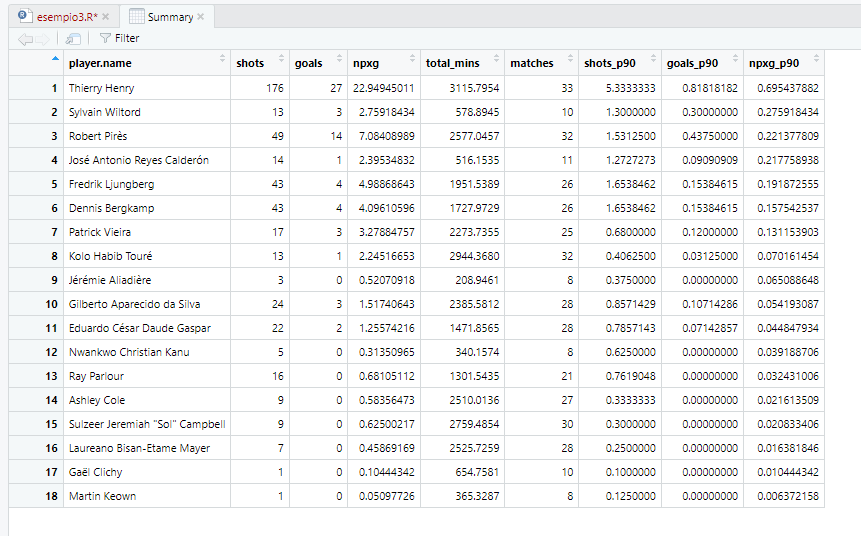
\includegraphics[scale=0.45]{Summary.png}
                \centering
                \caption{Dataframe Summary}
                \label{fig:Summary}
            \end{figure}

            \vspace{10pt}

            Anche in questo caso, si decide di omettere il codice per la presentazione dei prossimi grafici, in quanto si ritiene il codice privo di rilevante significato. Il primo grafico che si intende proporre è uno scatterplot che relaziona i goal segnati e tiri effettuati da ciascun giocatore nell'arco di una partita. Si ricorda che i punti plottati sono relativi a giocatori che hanno disputato almeno 6 partite nel campionato 2003/2004. Il grafico, presente in figura \ref{fig:RPlot06} è stato suddiviso in maniera arbitraria in 4 quadranti da due assi perpendicolari. 
            
            Intuitivamente, l'ideale per un giocatore sarebbe trovarsi nel quadrante in basso a destra, dal momento che significherebbe effettuare pochi tiri e allo stesso tempo realizzare molti goal. In effetti, non vi sono punti in tale regione proprio perchè è molto difficile trovare giocatori che rispecchino delle performance simili, come detto poco fa. Molto più comune, invece, è trovarsi nel quadrante alto a destra, in cui a tanti tiri corrispondono anche tanti goal. Qui vi sono tre giocatori, per i quali si è deciso di riportarne il nome, ad esempio il giocatore "Thierry Henry" ha effettuato in media poco più di 5 tiri a partita, segnando poco più di 0.8 goal a partita. Con un po' di approsimazione si può affermare che su ogni 5 tiri ha segnato 1 goal nell'arco del campionato 2003/2004. Il quadrante basso a sinistra contiene la maggior presenza di giocatori, i quali hanno effettuato tutti meno di 1 tiro in media e meno di 0.2 goal a partita. Probabilmente si tratta di calciatori che hanno un ruolo per il quale si trovano geograficamente lontani dalla porta avversaria, rendendo il gesto tecnico del tiro molto poco frequente per loro. Le stesse considerazioni valgono per il quadrante in alto a sinistra, con l'unica differenza che qui vi sono testimonianze di giocatori che hanno effettuato qualche tiro in più.

            \begin{figure}[h]
                \includegraphics[scale=0.35]{RPlot06.png}
                \centering
                \caption{Scatterplot Goals vs Shots per partita}
                \label{fig:RPlot06}
            \end{figure}

            Per il prossimo grafico, si considerano i top 3 calciatori con NpxG più alta del dataframe \texttt{Summary}, ovvero i giocatori presenti nel quadrante in alto a destra della figura \ref{fig:RPlot06}. Si estraggono anche le informazioni sulla posizione dalla quali i tiri sono partiti e per ciascun tiro, anche se poi è risultato un goal o meno.

            \vspace{10pt}

            \begin{lstlisting}[numbers=None]
    #We will consider the top3 players by NpxG
    Summary<-Summary %>% 
      slice(1:3)
    
    
    #filter location data by top 3 players, considering only shots
    shot_data <- Events %>% 
      filter(player.name %in% unique(Summary$player.name),
             type.name == "Shot") %>% 
      mutate(is_goal = ifelse(shot.outcome.name == "Goal", 1, 0) %>% 
               as.factor()) %>% 
      select(player.name, location.x, location.y, is_goal, shot.outcome.name, shot.statsbomb_xg, team.name)
            \end{lstlisting}

            \vspace{10pt}

            Il grafico di figura \ref{fig:RPlot07} esprime, per ciascuno dei tre giocatori con NpxG più alta, i tiri (no calci di rigore) che sono stati effettuati nel corso del campionato. Ciascun pallino corrisponde a un tiro e come si può notare in legenda, il colore discrimina un goal da un tiro che non è risultato in un goal. La grandezza dei pallini è riferita alla misura expected goal: quanto più un pallino è grande, quanto più e facile che il tiro si trasformi in rete e ciò spiega a grandi linee il fatto che i pallini vicino alla porta siano più grandi, mentre più ci si allontana, più diventano piccoli. Quanto appena detto non è del tutto vero, essendoci molti altri fattori che influenzano la xG, come ricordato sopra. Risulta molto interessante notare come la NpxG per partita non sembra essere influenzata in maniera pesante dai tiri e dai goal per partita, dal momento che il calciatore "Robert Pirès" ha la NpxG più bassa tra i 3 ma anche la percentuale realizzativa migliore tra i 3 in relazione ai tiri effettuati (circa 1 rete ogni 3.5 partite, a fronte di 1 rete ogni circa 4 partite per "Sylvain Wiltord" e 1 rete ogni circa 5 partite per "Thierry Henry"). Appare altrettanto evidente che "Thierry Henry" abbia la NpxG più alta probabilmente perchè ha segnato goal da una distanza maggiormente significativa dalla porta rispetto agli altri due calciatori, tant'è vero che i pallini verdi relativi alle reti più distanti dalla porta avversaria sono molto piccoli, segno del fatto che la xG in quei tiri è molto bassa. Un'ulteriore testimonianza a favore di quanto appena detto può essere legata al fatto che le reti segnate dagli altri due calciatori avevano xG alta e quindi erano tiri difficili da sbagliare e ciò non ha contribuito in maniera significativa sulla media stagionale. Altrettanto interessante è notare come il pallino in basso a destra nel grafico del calciatore "Thierry Henry" (non trasformato in rete) abbia una xG relativamente alta se si pensa alla distanza e angolatura dalle quali il tiro è partito. Più precisamente, un campo da calcio ha dimensioni che variano da un minimo di 45*90 metri a un massimo di 60*120 metri. Questo significa che il pallone, è stato calciato da metà campo, quindi da un range che va da 45metri a 60 metri dalla porta avversaria. 

            \vspace{10pt}
            
            \begin{figure}[h]
                \makebox[\textwidth][c]{\includegraphics[scale=0.8]{RPlot07.png}}
                \centering
                \caption{Top 3 calciatori con NpxG più alta}
                \label{fig:RPlot07}
            \end{figure}

            \vspace{5pt}

            \subsubsection{Approfondimento sulla metrica xG}
                L'ultima osservazione fatta per il grafico precedente incuriosisce particolarmente, a tal punto che in questa sotto-sezione si vuole presentare qualche dettaglio in più per quanto riguarda la metrica expected goal (xG). Di seguito si vuole evitare di spiegare quanto detto già sulla xG a livello introduttivo, l'obiettivo qui è cercare di capire qualcosa in più sui modelli che generano tale misura di probabilità. A tal proposito, non sono presenti fonti che spiegano "cosa c'è sotto" alla xG nella pagina di StatsBomb \cite{StatsBomb} ed è comprensibile che sia così. Probabilmente sfrutteranno modelli che hanno creato per conto loro e che non vogliono diffondere ai competitors. 

                A tal proposito in rete, è presente un articolo interessante che ha poco meno di un centinaio di citazioni, redatto dall'Università di Alicante (Spagna) riguardo tale metrica, reperibile a fondo pagina qui \cite{Articolo}. L'obiettivo dello studio in tale articolo, come riportato nell'abstract, è quello di analizzare i fattori che influiscono sulla xG. L'articolo dimostra come l'impiego della combinazione di entrambe le variabili distanza e angolatura dalla porta fornisce una stima più accurata dell'utilizzo di solamente una delle due. Inoltre, spiega anche come tale metrica permette di capire se una squadra sta over-performando o under-performando e, con ogni probabilità, le stesse considerazioni si possono fare per singoli giocatori. Lo studio fa notare che sono stati pubblicati molti post su blog e articoli da parte di statistici riguardo ai modelli per il calcolo di xG, in cui i modelli coinvolgono numerosi fattori oltre alla distanza e l'angolazione dalla porta, come ad esempio: velocità della palla durante il tiro, piede con cui la palla è stata calciata e infatti, ciascun calciatore ha un piede preferito con il quale si trova più sicuro quando deve calciare la palla, e persino gli scarpini con i quali è stata calciata la palla. Tutti questi studi presentano risultati molto contrastanti e ne consegue che non esiste un modello "generale" che permetta di misurare con accuratezza quali siano i fattori più influenti sul calcolo dell'xG.

                In ogni caso, ciò che viene marcato come importante nello studio, è che la predizione gioca un ruolo fondamentale e pertanto è stato usato un modello di regressione logistica sul dataset considerato. Lo studio pone l'accento sul fatto che l'aggiunta della combinazione delle due variabili distanza e angolazione non ha prodotto risultati migliori, nonostante non vi siano problemi legati al dataset. L'autore suppone che il principale candidato al problema sia stato il fatto di non aver considerato l'azione precedente che ha prodotto il tiro, ovvero il modo in cui la palla è giunta al calciatore che ha effettuato il tiro, come ad esempio calci d'angolo, calci di punizione e passaggi filtranti. L'autore sostiene che le tre variabili sono componenti importanti nella creazione di un modello e quindi sulla base dei dati forniti, un test statistico basato sulla regressione logistica non potrebbe essere impiegato. 
                
                Per compiere lo studio, sono stati analizzati i campionati inglese (Premier League) e tedesco (Bundesliga), il campo di gioco è stato suddiviso in aree a cui, per ciascuna zona, è stato applicato un valore di goal teorico, come si può notare in figura \ref{fig:Pitch}. I tiri sono stati raggruppati per area e i fattori analizzati sono stati principalmente la distanza e l'angolazione di tiro dalla porta. Successivamente, sono stati calcolati valori e relative percentuali in merito a tiri totali, tiri finiti sul bersaglio (porta avversaria), goal dalla zona di riferimento e infine xG, considerando i valori percentuali legati al numero di goal sui tiri totali per ciascuna zona e i tiri verso la porta per zona.

                \vspace{10pt}

                \begin{figure}[h]
                    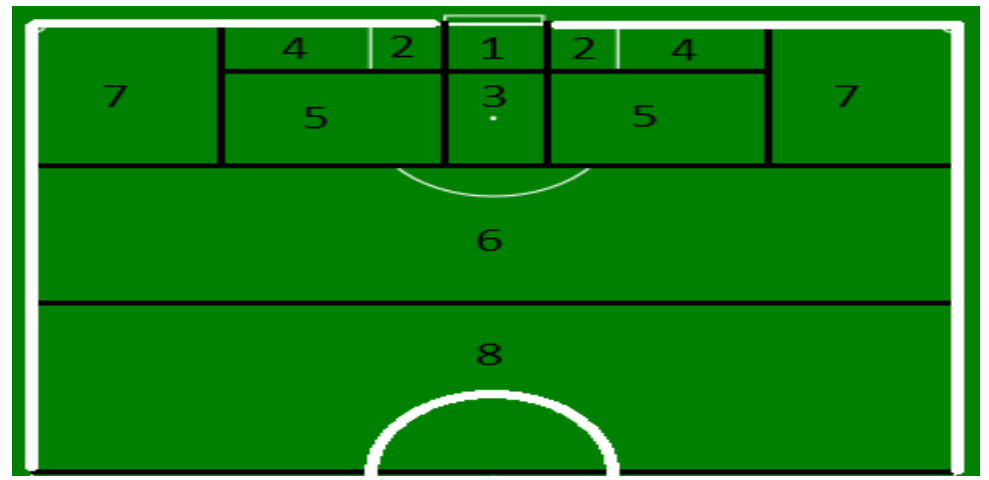
\includegraphics[scale=0.35]{Pitch.png}
                    \centering
                    \caption{Suddivisione campo in zone}
                    \label{fig:Pitch}
                \end{figure}
                
                \vspace{10pt}
                
                Lo studio termina sostenendo che la tesi relativa al fatto che la distanza dalla porta fornisce una stima sufficientemente accurata di xG si ritiene rigettata e inoltre, cosa più importante, i risultati del calcio sono difficili da prevedere correttamente e xG non fa di certo eccezione. Il numero di variabili che possono essere contate (stili di gioco, calci di punizione, colpi di testa, tipi di passaggio e dribbling) è infinito e avranno tutte un certo impatto sul totale xG di un giocatore (alcuni più di altri). Vale anche la pena notare che le dimensioni del campo dello stadio di ogni club sono diverse e questo fattore può anche influire sull'accuratezza di un tiro.
